\chapter{Aplicación Meteorológica.}\label{sec:AplicacionMeteorologica}

\paragraph{}En este capítulo se va a exponer toda la documentación técnica del diseño
y la arquitectura del software de la aplicación que usaremos de ejemplo para utilizar
el entorno de desarrollo.

\begin{figure}[H]
	\centering
	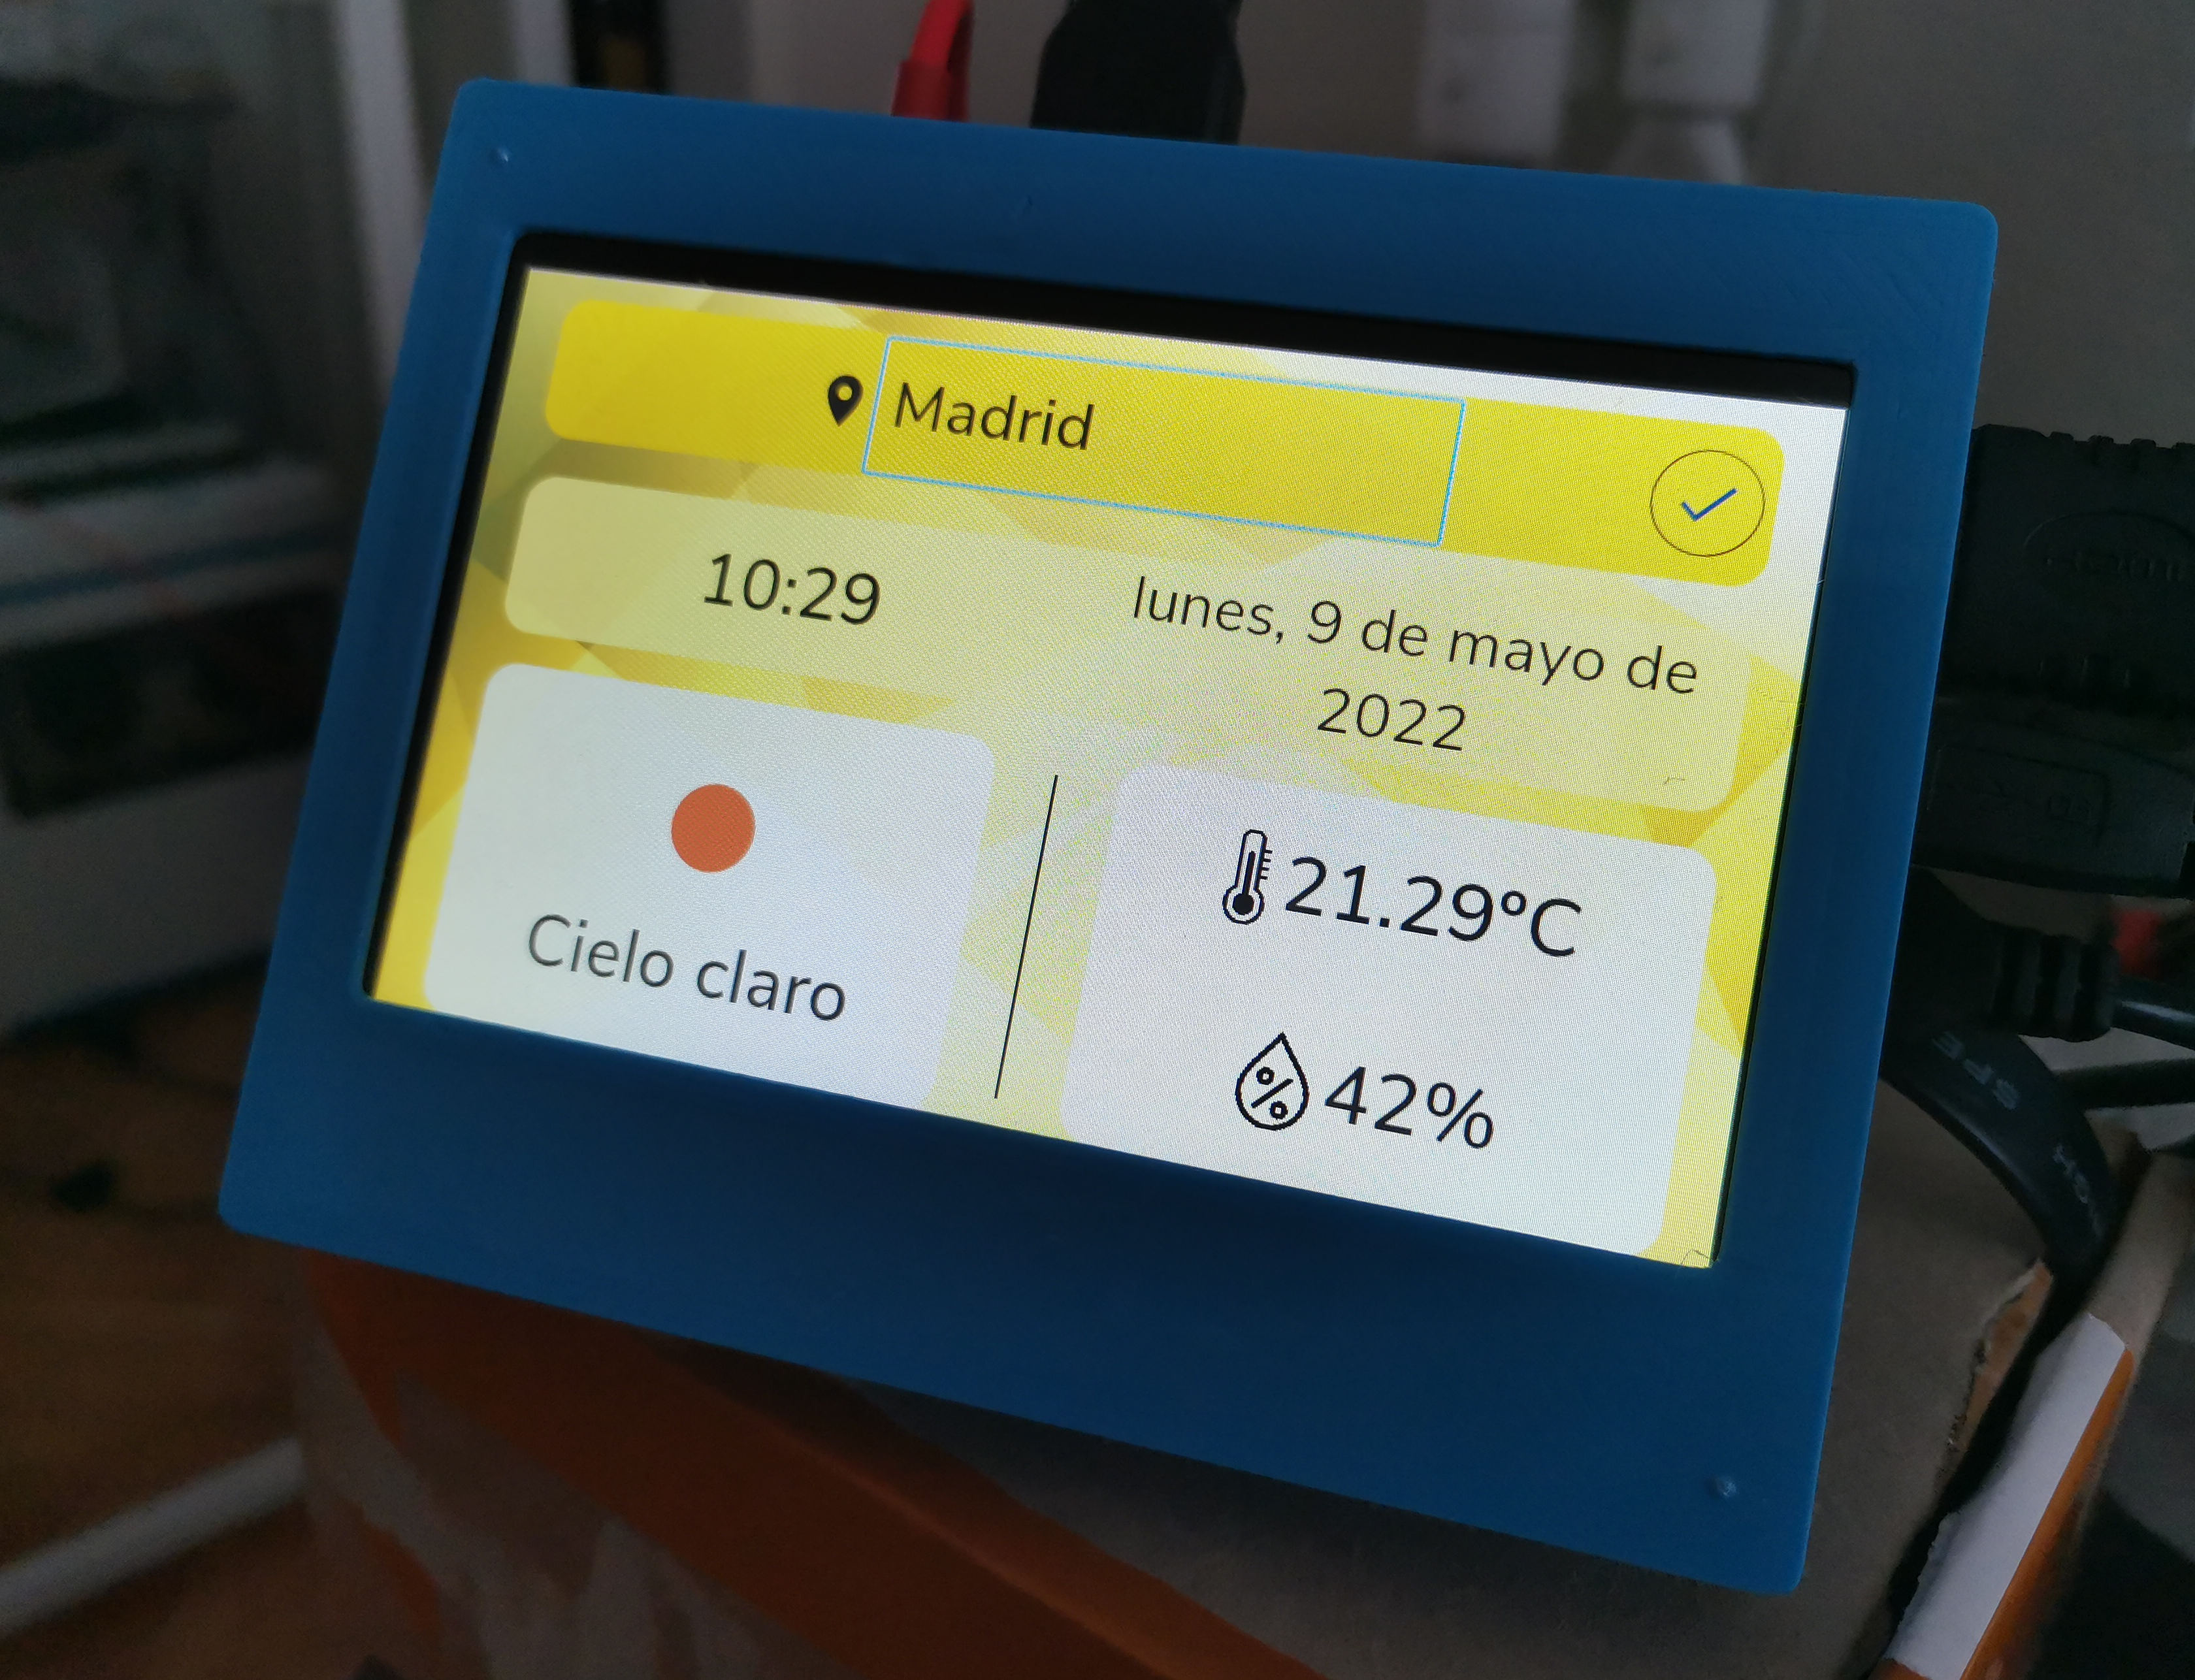
\includegraphics[width=0.9\linewidth]{imgs/app1}
	\caption[Portada de la app]{Fotografía de la aplicación en ejecución.}
	\label{img:rpi-weather-portada}
\end{figure}

\section{Requisitos}

\paragraph{}En esta sección se describirán los requisitos utilizados para el diseño
de la aplicación.

\subsection{Requisitos de usuario:}
\begin{itemize}
    \item Como usuario, quiero disponer de la fecha y hora en todo momento.
    \item Cómo usuario, quiero disponer de la información meteorológica de cualquier
    ciudad del mundo.
    \item Como usuario, quiero poder elegir la ciudad de la que quiero conocer la
    información meteorlógica.
\end{itemize}

\subsection{Requisitos funcionales:}
\begin{itemize}
    \item Se debe mostrar la información con la fecha, la hora y la información meteorlógica
    en todo momento.
    \item Como información meteorológica se debe mostrar: temeperatura, humedad, icono
    y breve descripción del estado actual.
\end{itemize}

\subsection{Requisitos no funcionales:}

\subsubsection{Requisitos de precisión:}
\begin{itemize}
    \item La hora mostrará horas y minutos en formato: HH:MM.
    \item La fecha debe mostrar: día de la semana, día del mes, mes y año.
    \item La temperatura se mostrará en grados centígrados con dos decimales de precisión.
    \item La humedad se representará con números enteros en tanto por ciento.
\end{itemize}

\subsubsection{Requisitos de rendimiento:}
\begin{itemize}
    \item La información debe actualizarse con una frecuencia mínima de 10 segundos y
    siendo deseable una frecuencia aproximada de 1 segundo.
\end{itemize}

\subsubsection{Requisitos de disponibilidad:}
\begin{itemize}
    \item La información debe mantenerse visible en todo momento mientras el sistema
    permanezca encendido.
    \item El sistema debe iniciarse tan pronto como se conecte a una fuente de energía.
\end{itemize}

\subsubsection{Requisitos de manejabilidad:}
\begin{itemize}
    \item La interfaz debe manejarse de manera táctil.
\end{itemize}

\subsubsection{Requisitos de recuperabilidad:}
\begin{itemize}
    \item Al encenderse, el sistema debe mostrar la información meteorológica de la
    última ciudad fijada.
\end{itemize}

\subsection{Requisitos de Interfaces externas:}

\subsubsection{Interfaces de usuario:}
\begin{itemize}
    \item Toda la información debe ser mostrada en un display de 5" táctil.
    \item El display permitirá el cambio de ubicación mediante uso del táctil de la pantalla.
\end{itemize}

\subsubsection{Interfaces de comunicaciones:}
\begin{itemize}
    \item El disposivo requerirá acceso a internet para obtener las métricas.
    \item El acceso a internet puede ser provisto por una interfaz ethernet (cableada)
    o Wi-Fi (sin cables).
\end{itemize}

\section{Casos de Uso}

\paragraph{}En esta sección se describen los casos de uso extraídos de los requisitos
mediante un diagrama formal SysML.

\begin{figure}[H]
	\centering
	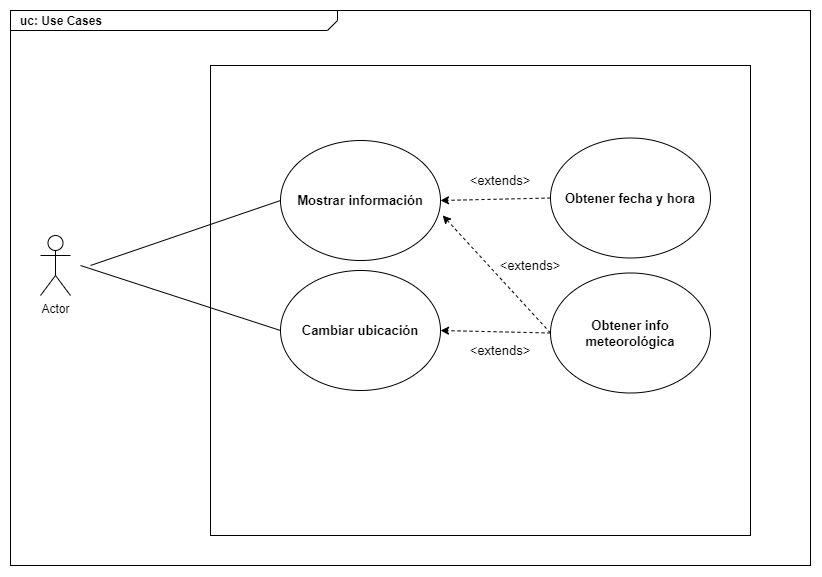
\includegraphics[width=0.9\linewidth]{figs/rpi_weather-uc}
	\caption[Diagrama SysML de casos de uso]{Diagrama SysML de casos de uso.}
	\label{fig:use_cases}
\end{figure}

\section{Diseño de interfaz de usuario}

\paragraph{}La interfaz de usuario en este caso se compone únicamente de una pantalla
táctil. Los diseños mostrados en esta sección, pertenecen al diseño original hecho en
Figma, un servicio online de diseño especializado en interfaces de usuario. Por eso mismo,
pueden existir pequeñas variaciones con el diseño final mostrado en la implementación final.

\clearpage
\paragraph{}\textbf{Pantalla principal:}

\begin{figure}[H]
	\centering
	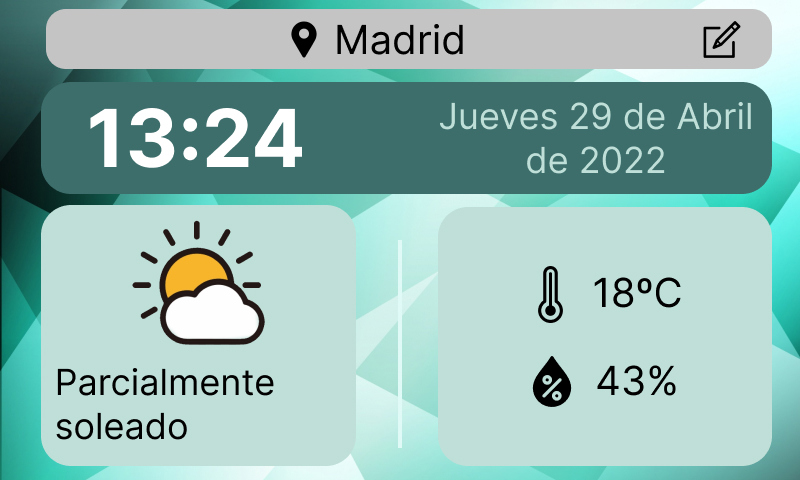
\includegraphics[width=0.75\linewidth]{imgs/figma-main}
	\caption[Diseño de la pantalla principal]{Diseño de la pantalla principal}
	\label{fig:design_main_screen}
\end{figure}

\paragraph{}\textbf{Edición de la localización:}

\begin{figure}[H]
	\centering
	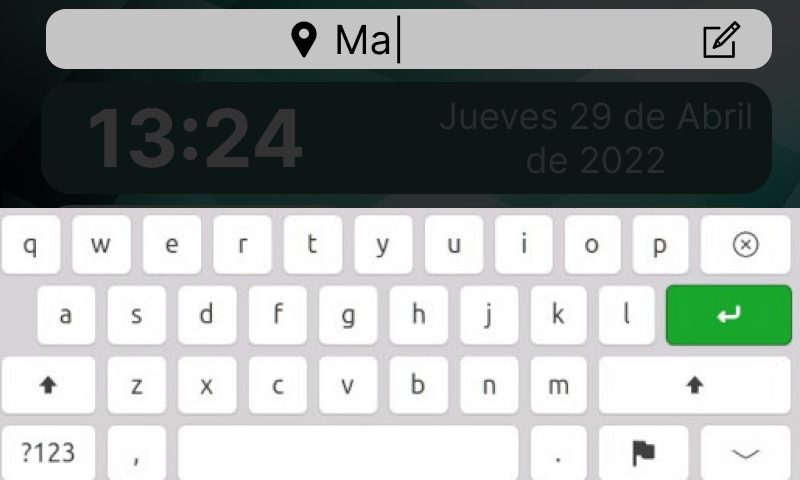
\includegraphics[width=0.75\linewidth]{imgs/figma-location}
	\caption[Diseño del cambio de localización]{Diseño del cambio de localización}
	\label{fig:design_location}
\end{figure}

\section{Arquitectura}

\paragraph{}La arquitectura de esta aplicación utiliza un patrón MVC modificado con el
patrón \emph{Change Notifier}. Esta arquitectura se caracteriza por manejar de forma
eficiente el estado de la aplicación. Las \emph{views} se suscriben a proveedores de
estado de los modelos que necesitan. Y cuando cambia el estado del modelo suscrito,
estas vistas se regeneran. Las vistas, a su vez pueden servir para cambiar el estado
de los modelos, previo tratamiento de los \emph{inputs} por la lógica de negocio provista
por los controladores.

\begin{figure}[H]
	\centering
	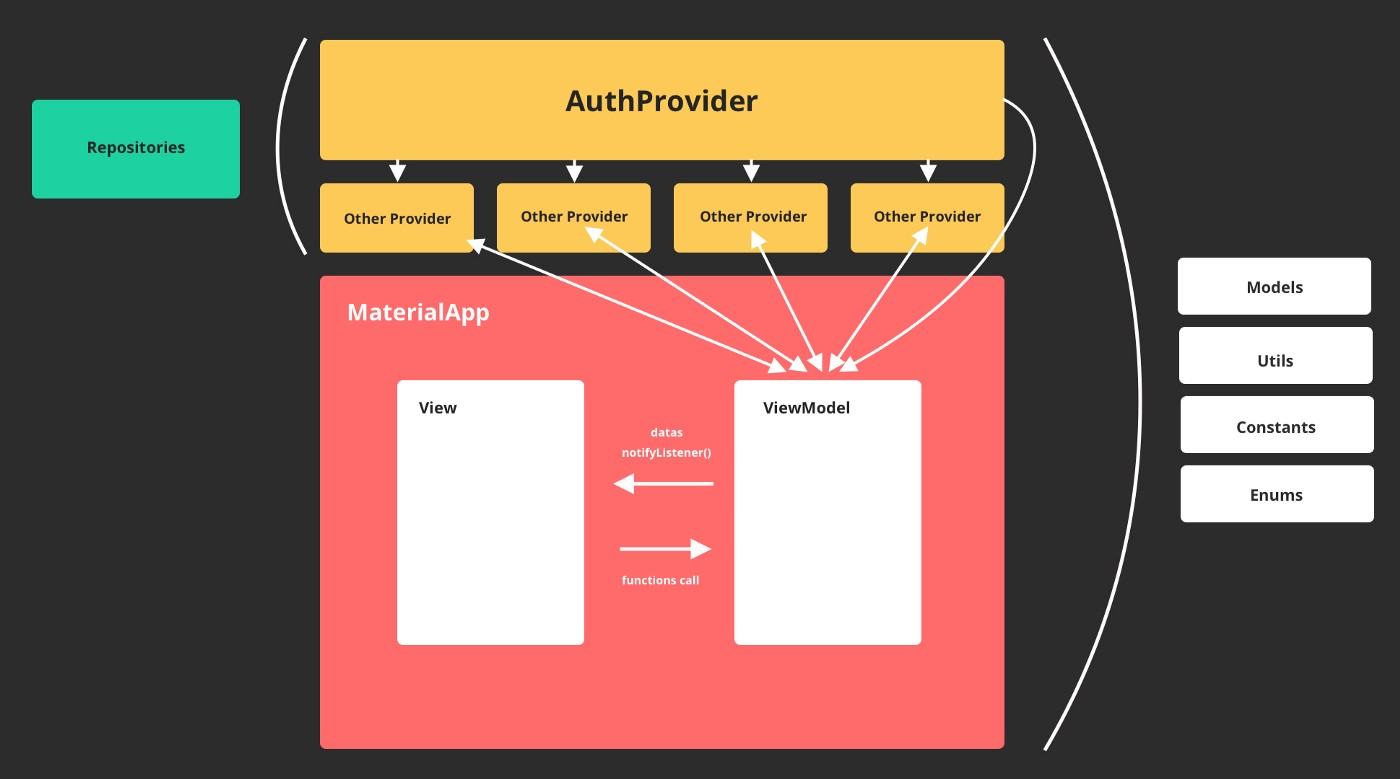
\includegraphics[width=0.85\linewidth]{figs/change-notifier}
	\caption[Arquitectura ChangeNotifier]{Diagrama de arquitectura Change Notifier.}
	\label{fig:ChangeNotifier}
\end{figure}

\paragraph{}En la figura \ref{fig:provider} mostrada a continuación, encontramos un
diagrama de clases genérico que explica como es la implementación del patrón de diseño
provider.

\begin{figure}[H]
	\centering
	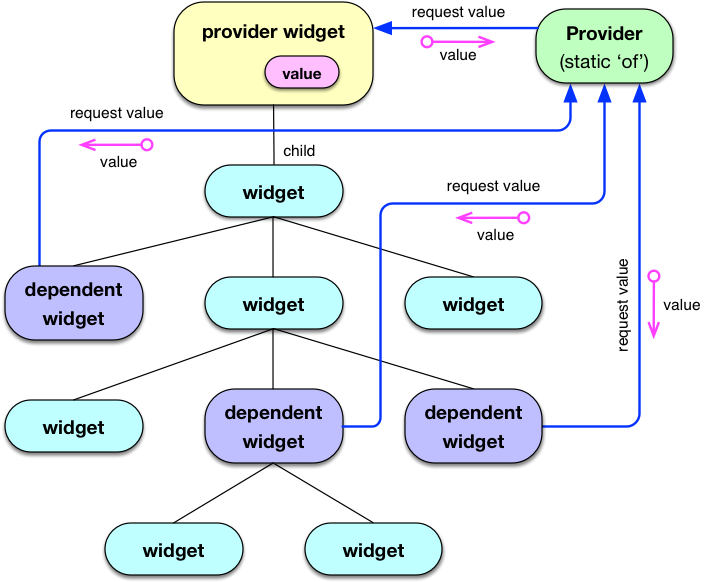
\includegraphics[width=0.75\linewidth]{figs/provider-pattern}
	\caption[Patron Provider]{Diagrama de clases con patrón provider.}
	\label{fig:provider}
\end{figure}

\subsection{Diagrama de clases}

\paragraph{}En la figura \ref{fig:classDiagram} se muestra el diagrama de clases de la
aplicación de meteorología implementada. El diagrama está algo simplificado para facilitar
la lectura y comprensión, sin embargo, representa fielmente la implementación.

\begin{figure}[H]
	\centering
	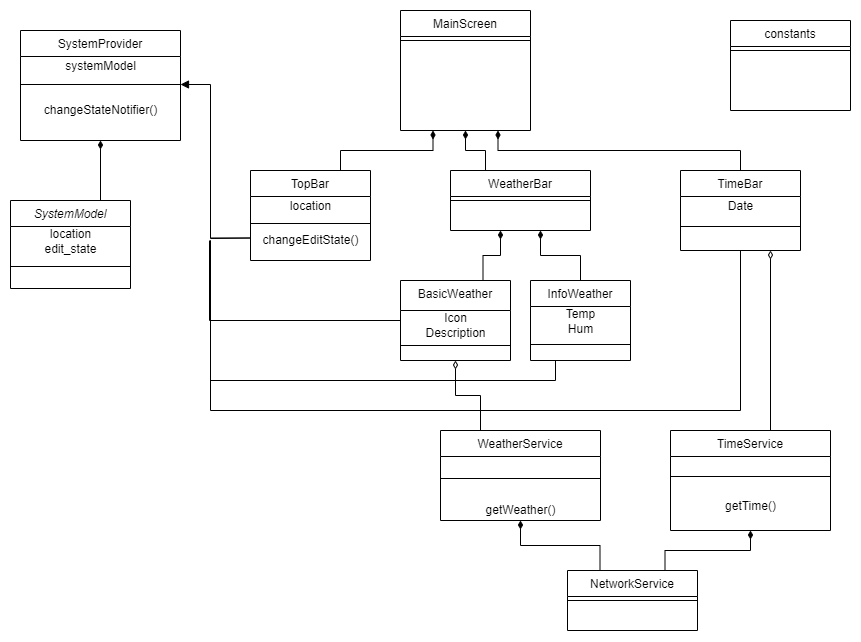
\includegraphics[width=0.95\linewidth]{figs/rpi_weather-class_diagram}
	\caption[Patron Provider]{Diagrama de clases con patrón provider.}
	\label{fig:classDiagram}
\end{figure}

\paragraph{}Como ya se ha dicho con anterioridad, esta aplicación se diseño para servir
de ejemplo o demostrador del entorno de desarrollo. El uso de aplicaciones flutter en
entornos embebidos y basado en Yocto no está muy extendido. No obstante, esto es sobre
todo debido a la falta de documentación, ya que queda demostrado cuan práctico y
conveniente puede llegar a ser.

\paragraph{}Al ser un demostrador,se ha querido documentar como si de una plantilla o
\emph{template} se tratase. También se han desarrollado unos cuantos test, para la
demostración del entorno de testing. Vale la pena recordar, que la aplicación en sí
misma es independiente del entorno de desarrollo y del proyecto Yocto que la usa.

\paragraph{}Todo el código de la aplicación y los comandos de uso básicos se pueden
encontrar en el siguiente repositorio de código público:

\paragraph{}\href{https://github.com/Gmatarrubia/rpi_weather}{github.com/Gmatarrubia/rpi weather}


%las referencias a artculos se ponen con \cite,
%las referencias a imgenes \ref,
%las referencias a glosario \gls,
%y las referencias a ecuaciones \eqref
